\documentclass{report}
\usepackage[T1]{fontenc}
\usepackage[utf8]{inputenc}
\usepackage[english]{babel}
\usepackage{graphicx}
\usepackage[hidelinks]{hyperref}
\usepackage{fancyhdr}
\pagestyle{fancy}
\lhead{\textbf{System and device programming}}
\rhead{Laboratory 6}
\lfoot{Enrico Franco}
\rfoot{Politecnico di Torino}
\author{Enrico Franco}
\title{System and Device Programming \\
	Laboratory 6 - Exercise 2}
\begin{document}
\section*{Exercise 2}
After installing the \texttt{chardev\_SDP\_lab} module it is needed to create a device as indicated in \texttt{/var/log/kern.log}. It is possible to read directly this file or to use command \texttt{dmesg} in order to see the output generated by the module itself, as shown in figure~\ref{img:dmesg_device_indication}.

\begin{figure}[hbtp]
\centering
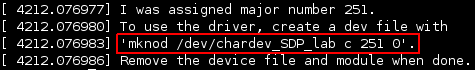
\includegraphics[scale=0.5]{images/es02/dmesg_device_indication.png}
\caption{Indication on where to create the device}
\label{img:dmesg_device_indication}
\end{figure}

By simply copying the highlighted line, it is possible to create the device and verify that it has been created using command \texttt{ls}, as shown in figure~\ref{img:mknod}.

\begin{figure}[hbtp]
\centering
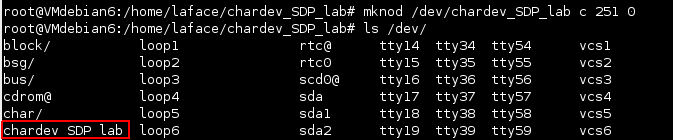
\includegraphics[scale=0.5]{images/es02/mknod.png}
\caption{mknod}
\label{img:mknod}
\end{figure}

After compiling \texttt{test\_chardev.c} file, it is possible to test (partially) the correct behavior of the device. In fact, characters are correctly sent to device, stored and sent back from it, as shown in figure~\ref{img:test_chardev}.

\begin{figure}[hbtp]
\centering
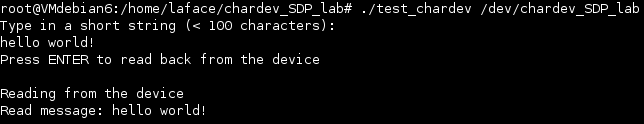
\includegraphics[scale=0.5]{images/es02/test_chardev.png}
\caption{test\_chardev.c behavior}
\label{img:test_chardev}
\end{figure}

Initially, the device does not behave as expected with commands \texttt{echo} and \texttt{cat}, as shown in figure~\ref{img:test_cat_01}.

\begin{figure}[hbtp]
\centering
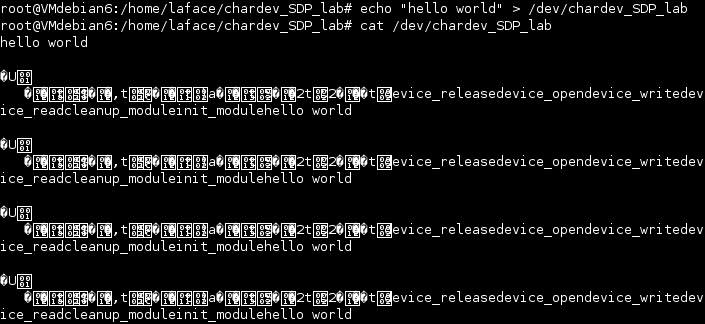
\includegraphics[scale=0.4]{images/es02/test_cat_01.png}
\caption{Initial cat behavior}
\label{img:test_cat_01}
\end{figure}

In fact, \texttt{cat} is implemented as a cycle, therefore until \texttt{device\_read} returns a number greater than 0, it will continue to read. Hence, it is needed to return 0 when the buffer is empty and to do this, it is needed to track the buffer size, e.g.\@ \texttt{global\_counter}, by incrementing it when some characters are written and decrementing it when some characters are read.

\texttt{device\_write}, instead, which is called by an \texttt{echo}, returns the number of correctly written characters. Therefore, it should return an error code if it is not possible to write on the device. Its role is to append new characters to the existing ones avoiding buffer overflow, e.g.\@ when \texttt{count} + \texttt{global\_counter} is greater than \texttt{BUFLEN}. 

After these modification, device driver works as expected on single \texttt{echo} and single \texttt{cat}, as show in figure\ref{img:echo_ok}.

\begin{figure}[hbtp]
\centering
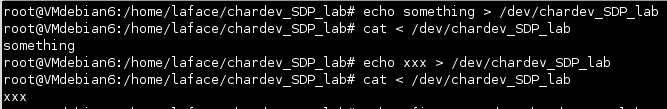
\includegraphics[scale=0.4]{images/es02/echo_ok.png}
\caption{Initial cat behavior}
\label{img:echo_ok}
\end{figure}

In order to avoid annoying \emph{newline} characters, they are removed from the device buffer before appending the new string, as show in figure~\ref{img:echo_multiline_ok}.

\begin{figure}[hbtp]
\centering
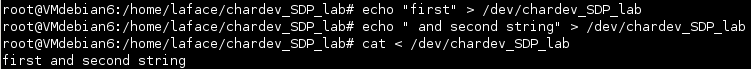
\includegraphics[scale=0.4]{images/es02/echo_multiline_ok.png}
\caption{Initial cat behavior}
\label{img:echo_multiline_ok}
\end{figure}

\end{document}